\message{ !name(SfM.tex)}\newcommand{\sig}{\sigma}
\newcommand{\Sig}{\Sigma}
\newcommand{\eps}{\epsilon}
\newcommand{\del}{\delta}
\newcommand{\ah}{\alpha}
\newcommand{\lam}{\lambda}
\newcommand{\gam}{\gamma}
\newcommand{\kap}{\kappa}
\newcommand{\rarr}{\rightarrow}
\newcommand{\larr}{\leftarrow}
\newcommand{\Rarr}{\Rightarrow}
\newcommand{\Larr}{\Leftarrow}

\newcommand{\ol}{\overline}
\newcommand{\dagg}{\dagger}
\newcommand{\mbb}{\mathbb}
\newcommand{\contra}{\Rightarrow\Leftarrow}
% for cross product
\newcommand{\lc}{\langle} %<
\newcommand{\rc}{\rangle} %>
% linear alg
\newcommand{\inv}{^{-1}}
\renewcommand{\vec}[1]{\boldsymbol{#1}}
\newcommand{\kth}{^{(k)}}
% order 
\newcommand{\cO}{\mathcal{O}}
% gradient
\newcommand{\grad}{\nabla}
\newcommand{\ddx}{\frac \partial {\partial x}}

%other shortcuts
\newcommand{\ben}{\begin{enumerate}}
\newcommand{\een}{\end{enumerate}}
\newcommand{\beq}{\begin{quote}}
\newcommand{\enq}{\end{quote}}
\newcommand{\hsone}{\hspace*{1cm}}
\newcommand{\hstwo}{\hspace*{2cm}}

\newcommand{\noi}{\noindent}
\parskip 5pt
\parindent 0pt

\documentclass[a4paper]{article}
\usepackage{amsmath,amssymb,hyperref,graphicx}
\begin{document}

\message{ !name(SfM.tex) !offset(-3) }

\title{Affine Structure from Motion}
\author{Scientific Computing CS660 Fall '11 Final Project \\ Angjoo Kanazawa}
\date{\today}
\maketitle

\section{Introduction}
Over the last few decades, the influence of Scientific Computing has
been so prevelent in almost every area of Science and Engineering. It has
become a necessary and critical tool for anyone involved in high-level
research in Computer Science. Computer Vision is one of the quintessential example of a research area that heavily builds upon
methods discovered in Scientific Computing, where the primary interest
lies in the analysis and understanding of images which are represented
in numerical matrices. This project explores applications of
computational algorithms explored in Scientific Computing via tackling
the problem of 3D reconstruction of an object from a stream of images.

The 3D reconstruction problem consists of a series of challenges starting from developing the
cameral model and feature representation of the image,
tracking such features over the image sequences , and finally
reconstructing the 3D geometry from the tracked points. In all of these steps,  The application of algorithms explored in
Scientific Computing is ubiqutous in all of these steps. 

The main challenge of recovering 3D geometry of objects and camera motion simultaneously from a set of point
correspondences is referred to as the Structure from Motion (SfM) problem. The solution to the problem has a
wide range of application in 3D modelling, virtual and augmented
reality models in computer graphics, camera calibration and many
more. It is a well studied problem with various approaches; this project focuses on the \emph{factorization} method proposed by Tomasi and Kanade
\cite{Tomasi} under the orthographic camera projection model. The
algorithm provides a numerically stable closed from optimal solution
via the singular-value decomposition technique under certain
conditions. \cite[p. 435]{AZ}

This project follows the Project 4 of Derek Hoiem's CS 543/ECE 549
course at the University of Illinois at Urbana-Champaign:
\href{http://www.cs.illinois.edu/class/sp11/cs543/hw/hw4.pdf}{project
  description}. 

\section{Background}

\subsection{Orthographic Projection}
\label{sec:ortho}
A camera model transforms a world point into an
image point. An affine camera, often used for
its simplicity, preserves up to affine transformation of world points
to image points. Basically it is a linear mapping followed by a translation, where
points can rotate, scale, and translate but parallelism is
preserved.\cite[p.38]{Szelski}. 
% \begin{figure}[!ht]
%   \begin{center}
%   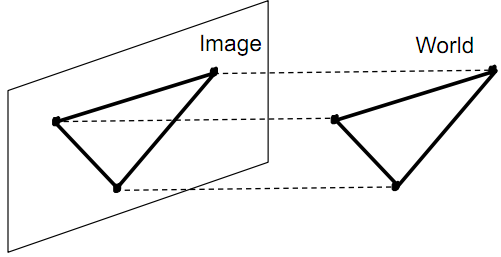
\includegraphics[scale=0.6]{ortho.png}
%   \caption{Orthographic Projection} 
%   \label{figures:ortho}
%   \end{center}
% \end{figure}
An \emph{orthographic
camera model} is a specific type of affine camera where the world
points are projected in parallel onto the image plane, where the depth
information of the world $Z$, is simply ignored. Mathematically, 
\begin{align*}
\begin{pmatrix}
  x\\y
\end{pmatrix} &= \begin{pmatrix}
  1& 0&0 \\0 & 1 & 0
\end{pmatrix}
R
\begin{pmatrix}
  X\\Y\\Z\\
\end{pmatrix} + \vec t\\
\vec x &= M\vec X + \vec t
\end{align*}
Where $M = \begin{pmatrix}
  1& 0&0 \\0 & 1 & 0
\end{pmatrix}R \in \mathbf{R}^{2\times 3}$ is referred to as the projection matrix, and $R$
is a 3 by 3 matrix representing the affine motion (rotation, translation, or
both) of the camera and $t$ is the displacement vector
\cite[p.172]{AZ}. In another words $M$ encapsluates the motion of the
camera under orthography.

\subsection{Notations and Assumptions}
\label{sec:notations}
A ``world point'' refers to a point, in the 3D
coordinate system, $\vec X = (X,Y,Z)^T$, and an ``image point'' refers
to a point projected on to an image plane in the 2D coordinate system,
$\vec x =(x,y)^T$. 

$I(x,y)$ denotes the pixel intensity value of image $I$, and $I(x,y,t)$ denotes the
pixel value of image $I$ at time $t$. $\grad I$ is the image gradient
$[I_x  I_y]$ and $H$ is the image hessian $\begin{pmatrix}  I_x^2
  & I_xI_y \\ I_yI_x & I_y^2\end{pmatrix}$

In this project, all projections are orthographic \ref{sec:ortho}
and the camera motion is affine. The images are assumed to have a mean-zero Gaussian noise. The world projected on the image
sequences is rigid and the pixel intensities of images over sequences are
constant i.e. all frames taken under static environment with no
brightness changes. Also for the experiment we assume that there is
no occlusion.

\subsection{Problem Statement}
\label{sec:problem-statement}
Given $F$ frames of sequencial images (videos), obtain $P$ trajectory
of image points for all $F$: $\{x_{fp} = (u_{fp}, v_{fp})^T
\forall F, P$ and solve for $X_{p}$, the world coordinate of all $P$ points.
these observation. 
For the experiments, the hotel image stream used in the original
Tomasi and Kanade paper was used. Frames 1, 15, 30, and 45 are
in figure \ref{fig:hotel}. 
% \begin{figure}[!ht]
%   \begin{center}
%   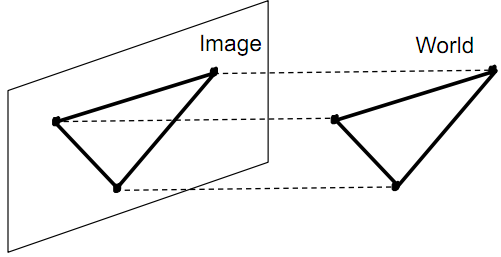
\includegraphics[scale=0.5]{ortho.png}
%   \caption{frames 1, 15, 30, and 45 of the hotel image stream} 
%   \label{fig:hotel}
%   \end{center}
% \end{figure}
\section{Structure for Motion}
\label{sec:main}
There are three main components for 3D reconstruction of an image stream. First we need to select a subset of
``interesting'' pixels from the original frame. These points are then
tracked through out the rest of the squence. This set of point
correspondence across all frames is then fed into the factorization algorithm. Appropriate keypoint selection and accurate feature tracking
are critical for a successful 3D reconstruction. 

\subsection{Keypoint Selection}
\label{sec:keypoint-selection}
It's not computationally possible to solve the world coordinate for every pixel of image sequences. We need to
select keypoints in the image that are reliable, salient, and
meaningful. 
% \begin{figure}[!ht]
%   \begin{center}
%   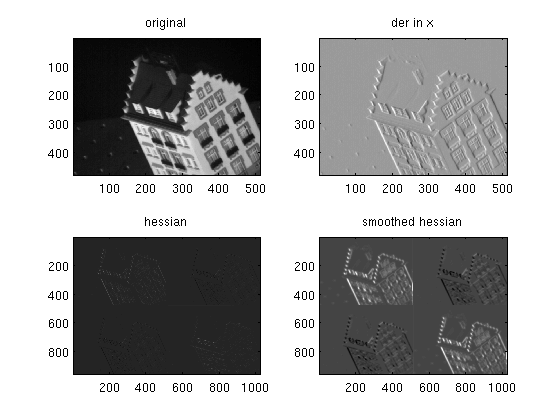
\includegraphics[scale=0.5]{hessian.png}
%   \caption{Plot of the image gradients of the first frame} 
%   \label{fig:Hessian}
%   \end{center}
% \end{figure}

\emph{Harris corner detector} is an optimal feature selection for the
tracker that is used for this project. (It's optimality is discussed
in section \ref{sec:feature-tracking}). The idea is that we should easily recognize an interesting point by looking through a
small window, where shifting a window in any direction
should give a large change in intensity i.e. we accept a point $\vec x$ if SSD of
the displacement of the window by $(u,v)^T$, $E(u,v) =
\sum_{(x,y)\in W} [I(x+u, y+v) - I(x,y)]^2$, is large in all
direction. 
Assuming $\vec d = (u,v)^T$ is small, the taylor series expansion of $I$ is
$$I(x+u, y+v) \approx I(x,y) + I_xu +I_yv + \cO(d^Td)$$ where $I_x
=\frac{\partial I}{\partial x} $, $I_y = \frac{\partial I}{\partial y}$.

Then, 
\begin{align*}
  E(u,v) &=\sum_{(x,y)\in W} [I(x+u, y+v) - I(x,y)]^2\\
&=\sum_{(x,y)\in W} [I(x,y) + I_xu +
I_yv - I(x,y)]^2\\
&= \sum_{(x,y)\in W} (
\begin{pmatrix}
  I_x & I_y
\end{pmatrix}
\cdot
\begin{pmatrix}
  u \\ v
\end{pmatrix}
)^2\\
&= \begin{pmatrix}
  u & v
\end{pmatrix} 
\begin{pmatrix}  I_x^2
  & I_xI_y \\ I_yI_x & I_y^2\end{pmatrix} \begin{pmatrix}
  u \\ v
\end{pmatrix}\\
&=d^T H d.
\end{align*}
  Since the two eigenvalues of $H$
,$\lam_1, \lam_2$, denotes the amount of change in the direction of its corresponding
eigenvector, we accept a window if $min(\lam_1, \lam_2) > \tau$, where
$\tau$ is predefined threshold \cite{shi}. Figure \ref{fig:Hessian} illustrates
the components of the Hessisan of frame one. 

Using the harris detector, X points were found on frame 1 of the hotel
sequence \ref{fig:keypoints}.
% \begin{figure}[!ht]
%   \begin{center}
%   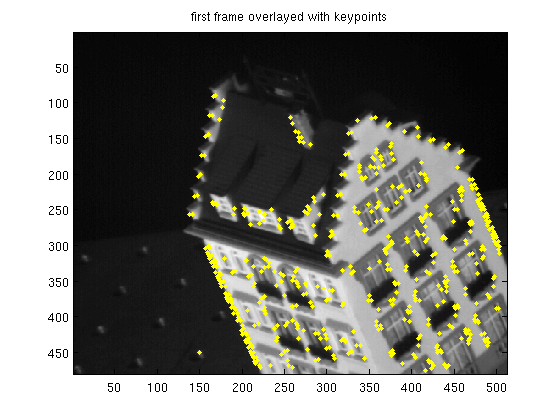
\includegraphics[scale=0.5]{keypoints.png}
%   \caption{First P keypoints found on frame 1} 
%   \label{fig:keypoints}
%   \end{center}
% \end{figure}

\subsection{Feature Tracking}
\label{sec:feature-tracking}
Now using the detected keypoint, we track these points over all frames
using the Kanade-Lucas-Tomasi (KLT) Tracker \cite{KLT}.
The basis of KLT tracker is that although image intensities change as
camera moves, images taken at near time are strongly related to each
other because they tend to refer to the same scene given the
assumption of local brightness constancy. This means that under an ideal
static environment, image at time $t+1$ can be obtained by moving
every pixel in the at time image $t$ by a suitable amount \cite{shi}. 

\subsubsection{Estimating Camera Motion}
This displacement can be either a translation or an affine mapping or
the combination of both, but since the world is rigid we will only
consider translation. Mathematically, given $\vec x$ at frame $t$, we
want to find a displacement vector, $\vec d=(u,v)^T$, that minimizes
the dissimilarity
\begin{equation}
  \label{eq:1}
 I(\vec x + \vec d, t+1) - I(\vec x, t) = 0
\end{equation}

The taylor expansion of $$I(\vec x+\vec d, t+1) = I(x+u, y+v, t+1) \approx I(x,y,t) + I_xu +
I_yv + I(x+u, y+u, t) + I_t \cO(d^Td).$$  Where $I_t$ is the temporal
gradient (for time) $I_t(\vec x) =I(\vec x, t) - I(\vec x+\vec d, t+1)$. Substituting that back to \eqref{eq:1},
\begin{align*}
0 &\approx I(x,y,t) + I_xu +I_yv  + I_t - I(x,y,t)\\
&= \grad I(\vec x)\cdot \vec d + I_t(\vec x)
\end{align*}
 Here we have 2
unknowns but only one constraint. In fact even with the brightness
constancy assumption, it is difficult to track a single point unless
the point is extremely distinctive \cite{KLT}. Therefore we consider minimizing
the dissimilarity within a small window (typically around 15 x 15) and
obtain an overdetermined linear system of equations:
\begin{align*}
\sum_{\vec x\in W} \grad I(\vec x) \cdot \vec d &= \sum_{\vec x\in W}
I_t \\
A\vec d &= \vec t
\end{align*}
Using the normal equations, we solve this least linear squares
problem:

\begin{align}  \label{eq:klt}
  A^TA\vec d &= A^T \vec t\\
  \begin{pmatrix}
    I_x(x_1) & \hdots & I_x(x_{|W|}) \\
   \vdots &  & \vdots \\
  I_y(x_1) & \hdots & I_y(x_{|W|}) \\
  \end{pmatrix}
  \begin{pmatrix}
    I_x(x_1) & \hdots &   I_y(x_1)  \\
   \vdots &  & \vdots \\
I_x(x_{|W|})& \hdots & I_y(x_{|W|}) \\
  \end{pmatrix}
\vec d  &= 
  \begin{pmatrix}
    I_x(x_1) & \hdots &   I_y(x_1)  \\
   \vdots &  & \vdots \\
I_x(x_{|W|})& \hdots & I_y(x_{|W|}) \\
  \end{pmatrix}
  \begin{pmatrix}
    I_t(x_1)\\ \vdots \\ I_t(x_{|w|})
  \end{pmatrix}\\
\begin{pmatrix}
\sum_{\vec x\in W}  I_x^2 &\sum_{\vec x\in W} I_xI_y\\ \sum_{\vec x\in
  W} I_y^2 &\sum_{\vec x\in W} I_yI_x
\end{pmatrix}
\begin{pmatrix}
  u \\ v
\end{pmatrix}
 &=
\begin{pmatrix}
 \sum_{\vec x\in W} I_xI_t\\ \sum_{\vec x\in W}I_yI_t
\end{pmatrix} \\
Z\vec d &= \vec e
\end{align}
% \begin{figure}[!ht]
%   \begin{center}
%   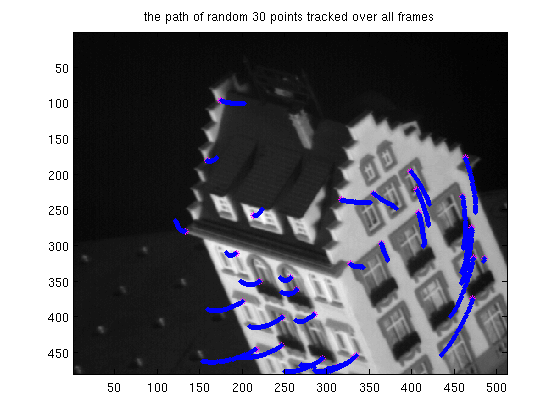
\includegraphics[scale=0.5]{tracked.png}
%   \caption{Plot of the random 20 points tracked over all frames} 
%   \label{fig:track}
%   \end{center}
% \end{figure}
Since solving for $\vec d$ by the method above requires us to konw
$I_t$, which requires an initial displacement $\vec d_0$, so we solve
for the verctor iteratively. Namely, we start with $\vec d_0
=(0,0)^T$ to compute $I_{t_0} = I(\vec x, t+1) - I(\vec x, t)$, then
solve for $\vec d_1$ using $I_{t_0}$. We iterate this until $||\vec
d_k - \vec d_{k+1}|| \le \delta$, $\delta$ some threshold.

Figure \ref{fig:track} is the tracked path of 20 random keypoints over
the entire sequence. The round circle is the position at frame 1.

\subsubsection{Numerical Stability}
\label{sec:numerical-stability}
Can we solve \eqref{eq:4} reliably? It seems like in practice, it's
not unusual to solve for $\vec d$ simply by taking the pseudo-inverse of $Z$,
which is known to be atrocious in the Scientific Computing
community. But there is a reason why here it is okay to be less
careful about solving for $\vec d$ and it leads to the discussion of
the optimality of our key point selecter.

For \eqref{eq:4} to be stable, w need $Z$ to be
well-conditioned. The condition number of $Z$ is $\kappa(Z) =
||A||||A\inv||$. Here, $Z$ is symmetric and positive definite (because
it's the Hessian), so the condition number is also the ratio of the
smallest to largest eigenvalue. Here it's $\frac{\lam_1}{\lam_2}$.
Note that our criteria for choosing our keypoint was $\min(\lam_1,
\lam_2) > \tau$. So we are assured that $\lam_2$ eigenvalue is
sufficiently large. Since we're dealing with images with a maximum
possible pixel value, we are also assured that $\lam_1$ will not be
arbitrarily large. So with this keypoint selection, we're guaranteed to
have a well conditioned $Z$. This is why in practice it is okay to use the pseudo-inverse
of $Z$. This means in MATLAB the \texttt{mldivide} is more than
sufficient.


\subsection{The Factorization Method}
As discussed in \ref{sec:ortho}, orthographic camera model projects
the world points onto the image plane as a linear mapping followed by
a translation: $x=MX + t$. Our goal is to esimate the camera motion
$M_f$ and $t_f$ for each frame and the world points, $X_p$, of all tracked
image points, so that the distance of the estimated image point from
these parameters and the measured image point is close. i.e. our
minimization problem is:
\begin{equation}
  \label{eq:fact}
\min_{M_f, t_f, X_p}\sum_{f}\sum_p ||x_{fp} - (M_fX_p + t_f)||^2  
\end{equation}
Taking the derivative of \eqref{eq:fact} with respect to $t_f$ and
setting it to 0 gives us $t_f = \bar x_f - M_f \bar X_p$, where $\bar
x_f =\frac{1}{P}\sum_p x_{fp}$ and $\bar X_p = \frac{1}{P}X_p$
i.e. the mean of all points in image $f$. But the origin of the world
point is arbitrary so we can just set that to 0, which gives us $t_f =
\bar x_f$. This also agrees with the fact that affine camera maps the
centroid of 3D world points to the centroid of the projected image
\cite[p438]{AZ}. This means that if we center all image points in $f$th
frame, $t_f=0$ and we can remove the translation term from the
model. Our objective is now: 
\begin{equation}
  \label{eq:fact2}
\min_{M_f, t_f, X_p}\sum_{f}\sum_p ||x_{fp} - M_fX_p||^2  
\end{equation}

The key idea of the factorization algorithm is that image measurements
can be decomposed into the product of two seperate factors
\emph{motion} and \emph{shape}. 

Using the set of $P$ tracked corresponding
points, we can represent the image sequence by a $2F\times P$ \emph{measurement matrix
}$$W =
\begin{pmatrix}
  x_{11} & \cdots & x_{1P}\\
  \vdots &  & \vdots \\
  x_{F1} & & x_{FP}\\
  y_{11} & \cdots & y_{1P}\\
  \vdots &  & \vdots \\
  y_{F1} & & y_{FP}\\
\end{pmatrix}
$$

Where $\vec x_{ij} = (x_{ij}, y_{ij})^T$ is the $j$-th point in the
$i$-th frame. 

Recall that camera motion under orthography is $$M_f =
\begin{pmatrix}
  i_f\\
  j_f
\end{pmatrix}
$$ where $i_f, j_f \in \mathbf{R}^{3}$, a pair of orthonomal unit vectors
corresponding to the x, y-axis of the image plane respectively. These vectors over $F$ frames are collected into a
\emph{motion matrix} $M\in \mathbf{R}^{2F \times 3}$ $$M =
\begin{pmatrix}
  i_1^T\\ \vdots \\  i_F^T \\ j_1^T \\ \vdots j_F^T
\end{pmatrix}
$$
We let $s_p = \vec X_p = (X_p, Y_p, Z_p)^T$ be the 3D coordinates of feature $p$ in the fixed world point with the same origin. These vectors are collected into a
\emph{shape matrix} $S\in \mathbf{R}^{3 \times P}$ s.t. $S =
\begin{pmatrix}
  s_1 & \cdots & s_p
\end{pmatrix}^T$. Using this notation, for a single frame we get
\begin{align*}
  \begin{pmatrix}
    x_{fp}\\y_{fp}
  \end{pmatrix} &=
  \begin{pmatrix}
    i_{f}^T\\j_{f}^T
  \end{pmatrix}
  \begin{pmatrix}
    X_p\\ Y_p\\ Z_p
  \end{pmatrix}\\
w_{fp} &= M_fS_p  
\end{align*}

So for all frames, we have the equation $$W = MS.$$
Our goal is to estimate $W$ by $\hat M$ and $\hat S$, where $\hat W = \hat M
\hat S$.
Now our objective can be re-written as a least squares problem:
\begin{equation}
  \label{eq:fact3}
\min_{M, S}||W - \hat M \hat S||^2
\end{equation}
\cite{Morita}.
\subsubsection{Rank Theorem}
Note that $W$ is the product of a $2F$ by $3$ motion matrix and
$3$ by $P$ shape matrix, therefore under ideal noise free environment,
$W$ is at most rank 3 \cite{Tomasi}. Assuming $2F \ge P$, we can
achieve the least squares approximation by factoring $W$ by SVD: $$W = U\Sigma V^T\\$$
Because of the rank theorem, the diagonal of $\Sigma$ has at most three nonzero
greatest singular values in the first three entries. So the closest approximation of $W$, even with noise,
is obtained by taking the three greatest singular values of $W$ with
the corresponding left and right eigenvectors. Namely,
\begin{align*}
W&\approx U_{2F\times 3}\Sigma_{3 \times 3} V_{3\times P}^T\\
&= \begin{pmatrix}
  u_{1,1} & u_{1,2} & u_{1,3} \\ \vdots & & \vdots
\\ \vdots & & \vdots
\\   u_{2F,1} & u_{2F,2} & u_{2F,3} 
\end{pmatrix}
\begin{pmatrix}
  \sigma_1 & 0 & 0 \\
  0 & \sigma_2 & 0 \\
  0 & 0 & \sigma_3 \\
\end{pmatrix}
\begin{pmatrix}
  v_{1,1} &  \cdots &\cdots & v_{1,p}\\
  v_{2,1} &  \cdots &\cdots & v_{2,p}\\
  v_{3,1} &  \cdots &\cdots & v_{3,p}\\
\end{pmatrix}
\end{align*}

By using SVD, the factorization algorithm achieves numerical stability
and we are guaranteed to converge to the global minimum of
\eqref{eq:fact3} \cite{Morris}. 

\section{Eliminating Affine Ambiguity}

One possible solution to estimate $\hat M$ and $\hat S$ is to choose
$\hat M = U_{2F\times 3}\Sigma_{3 \times 3}^{1/2}$ and $\hat S =\Sigma_{3 \times 3}^{1/2}V_{3\times P}^T$, or
$\hat M =U_{2F\times 3}$ and $\hat S=\Sigma_{3 \times 3}V_{3\times
  P}$, because either way we get $\hat W = \hat M \hat S = U_{2F\times 3}\Sigma_{3 \times 3} V_{3\times P}^T$

The approximation of $\hat M$ and $\hat S$ has such ambiguities, since
an arbitrary 3 by 3 invertible matrix $Q$ may be inserted in the
decomposition as $\hat W = (\hat M Q) (Q\inv \hat S)$, i.e. the
approximation is unique only upto an affine transformation. We can
upgrade this affine approxmiation to a metric approximation by
imposing the metric information obtained from the motion matrix $M$ to
solve for $Q$.

Let $$L = QQ^T =
\begin{pmatrix}
l_1& l_2& l_3\\
l_2& l_4& l_5\\
l_3& l_5& l_6\\
\end{pmatrix}
$$. Recall that $\hat M$ is made of orthonormal unit vectors where the first
$F$ entries of $\hat M$, $\hat i_f\in \mathbf{R}^3$, is orthogonal to the corresponding second $F$
entries of $M$, $\hat j_f \in \mathbf{R}^3$. Since $M = \hat M Q$, the corresponding
rows of $\hat M$ must satisfy equations 
\begin{align*}
  \label{eq:metric}  
  \hat i_f^T L \hat i_f &= 1\\
  \hat j_f^T L \hat j_f &= 1\\
  \hat i_f^T L \hat j_f &= 0.\\
\end{align*}

Stacking up elements of $L$ into a vector and re-writing the appropriate terms
we get an over-deteremined system of linear equations $G\vec l = \vec
c$, where $$
  G = \begin{pmatrix}
    f(\vec i_1, \vec i_1) \\ \vdots \\f(\vec i_F, \vec i_F) \\ \vdots \\
    f(\vec j_1, \vec j_1) \\ \vdots \\    f(\vec j_F, \vec j_F) \\ \vdots \\
    f(\vec i_1, \vec j_1) \\ \vdots \\f(\vec i_F, \vec j_F) \\ \vdots \\
  \end{pmatrix}\in \mathbf{R}^{3F\times 6}$$
 and $\vec c$ is a vector whose first $2F$ entries are 1 and the last
 $F$ entries are 0, and $f(\vec i_f, \vec j_f) = [i_{f1}j_{f1},
 i_{f1}j_{f2}+i_{f2}j_{f1}, i_{f1}j_{f3}+i_{f3}j_{f1}, i_{f2}j_{f2},
 i_{f2}j_{f3}+i_{f3}j_{f2}, i_{f3}j_{f3}]$.

We can solve for $\vec l$ using any least squares problem solver, then
employ cholesky decomposition to obtain $Q$ \cite{Morita}.

Finally we have $M = \hat MQ$, and $S =Q\inv \hat S$, where $S$
contains the 3D world point of the $P$ tracked points and $M$ has the
position of the camera over $F$ frames. 

Figure \ref{fig:3D} is the reconstructed 3D mesh of the hotel
sequence textured with the first image.
The camera position in each frame is given by the cross product of
$M_f$'s rows $\vec i_f \times \vec j_f$. The 3D path of camera
movement from each dimension is plotted on \ref{fig:path}.
% \begin{figure}[!ht]
%   \begin{center}
%   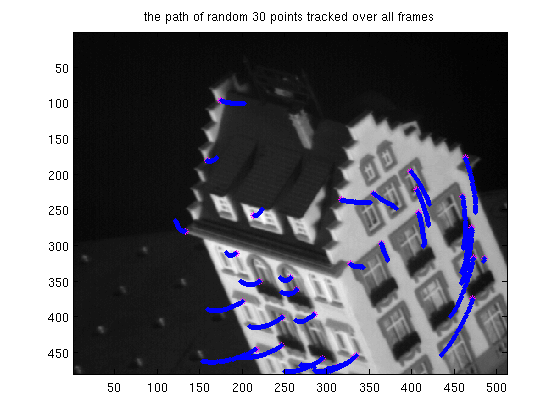
\includegraphics[scale=0.5]{tracked.png}
%   \caption{Plot of the random 20 points tracked over all frames} 
%   \label{fig:track}
%   \end{center}
% \end{figure}


% \begin{figure}[!ht]
%   \begin{center}
%   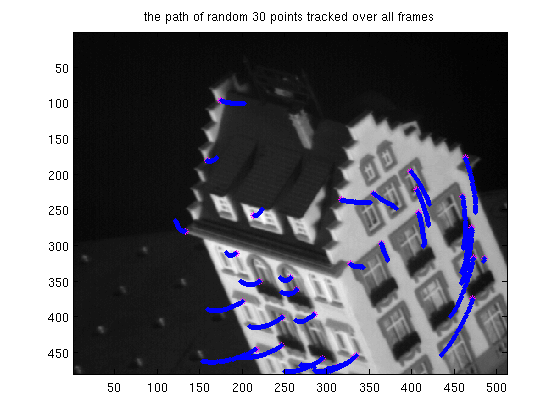
\includegraphics[scale=0.5]{tracked.png}
%   \caption{Plot of the random 20 points tracked over all frames} 
%   \label{fig:track}
%   \end{center}
% \end{figure}

\section{Conclusion}
\label{sec:conclusion}


The main challenge for Structure from Motion lies not in creating the
model of the system but in accurately estimating the parameters of the
model. Theoretically, an appropriate camera model's parameters are well-defined upto certain
ambiguities. However, the model is non-linear and has high sensitivity
to parameter variations which makes the problem numerically
ill-conditioned or computationally intensive in direct methods \cite{Morris}.

The main contribution of the factorization method is that under
orthography, the relationship between the measurement, the motion and
the shape matrix has a simple expression regardless of the shape or
the camera movement \cite{Tomasi}. The algorithm is alos numerically stable and the convergence to minimize the
norm squared error of the approximation of $W$ is guaranteed. Even
when the number of $F$ grows, there are methods to estimate $W$
efficiently because full SVD of $W$ is not necessary. 
The factorization method presented in this project assumes orthographic
projection but the algorithm has been further extended to work with
most camera models as well\cite{Morris}. 

Every step discussed above was implemented in MATLAB \ref{source}. As
proposed the method gives accurate reconstruction of the world
points. 

\appendix

\section{Source Code}
\paragraph{do\_SfM.m}
The driver.
\begin{verbatim}
function do_SfM(config_file)
%%%%%%%%%%
% CMSC660 Fall'11 Final Project: Affine Structure from Motion(SfM)
% doSfM.m
% Driver script to do affine SfM, to run, do:
% do_SfM('config'); where 'config' refers to the config.m in this directory
%
% Angjoo Kanazawa 11/23/'11
%%%%%%%%%%

%% Step 1: get initial keypoints

[keyXs, keyYs] = do_getKeypoints(config_file); 

%% Step 2: track features

[trackedXs, trackedYs] = do_trackFeatures(config_file);

%% Step 3: Affine Structure for Motion via Factorization

[M S] = do_factorization(config_file);
\end{verbatim}
\paragraph{do\_getKeypoints.m}
Code for section \ref{sec:keypoint-selection}
\begin{verbatim}
function [keyXs, keyYs] = do_getKeypoints(config_file)
%%%%%%%%%%
% getKeypoints.m
% script to get the key points from im using Harris corner detector
% INPUT - im: image to get the keypoint
%         tau: threshold to do non-maxima supression
%
% OUTPUT - keyXs, keyYs: keypoints found in the initial
% frame. saves them in the file specified by config.m
%
% parts of script referenced from: http://www.csse.uwa.edu.au/~pk/research/matlabfns/
%
% Angjoo Kanazawa 11/23/'11
%%%%%%%%%%

%% Evaluate the global configuration file and load parameters
eval(config_file);

imFiles  = getImageSet(IMAGE_DIR); % gets cell array of frames (img files)
F = length(imFiles); % number of frames
fprintf('getting intial keypoints from %s\n', imFiles{1});

im = double(imread(imFiles{1}));

if strcmp(Feature.method, 'harris')
    % compute image derivatives in x and y using Peter Kovesi's
    % accurate derivative
    [Ix Iy] = derivative5(im, 'x', 'y');
    % old way
    % dx = [ -1 0 1 ; -1 0 1 ; -1 0 1]; 
    % dy = dx';
    % Ix = imfilter(im, dx, 'same');
    % Iy = imfilter(im, dy, 'same');

    % compute components of H
    Ix2 = Ix.^2;
    Iy2 = Iy.^2;
    IxIy = Ix.*Iy ; 

    % smooth H using gaussian filter
    filt = fspecial('gaussian', 6*Feature.sigma, Feature.sigma);
    Ix2sm = imfilter(Ix2, filt, 'same');
    Iy2sm = imfilter(Ix2, filt, 'same');
    IxIysm = imfilter(IxIy, filt, 'same');

    % display plot
    % sfigure; subplot(2,2,1); imagesc(im); colormap('gray'); title('original');
    % subplot(2,2,2); imagesc(Ix); colormap('gray');title('der in x');
    % subplot(2,2,3); imagesc([Ix2 IxIy; IxIy Iy2]);colormap('gray'); title('hessian');
    % subplot(2,2,4); imagesc([Ix2sm IxIysm; IxIysm Iy2sm]);colormap('gray'); title('smoothed hessian');

    % compute the corner response matrix = det(H) - a*trace(H)^2
    M = Ix2sm.*Iy2sm - IxIy.^2 - Feature.alpha*(Ix2sm + Iy2sm).^2;

    % perform non-maxima supression over Feature.radius window size

    % Make mask to exclude points within Feature.radius of the image boundary. 
    bordermask = zeros(size(im));
    bordermask(Feature.radius+1:end-Feature.radius, Feature.radius+1:end-Feature.radius) = 1;
    % dilate image
    M_sup = ordfilt2(M, Feature.radius^2, ones(Feature.radius));
    % find points that's still there in dilated image & stronger than Feature.tau
    corner = (M==M_sup) & M>Feature.tau & bordermask;

    % plot
    if VERBOSE
        sfigure; subplot(221); imagesc(M); title('corner response M');
        subplot(222); imagesc(M_sup); title('max dilated');
        colormap('gray');
        subplot(223); imagesc(M> Feature.tau); title(['corner response > thresh']);
        colormap('gray');
        subplot(224); imagesc(corner); title('corner response max suppressed');
        colormap('gray');
    end

    [keyXs, keyYs] = find(corner); % get the r, c index of key points

else %do SIFT
   keyXs = [];
   keyYs = [];
end

if VERBOSE
    sfigure;
    imagesc(im); colormap('gray'); hold on;
    plot(keyYs, keyXs, 'y.');
    title(['first frame overlayed with keypoints']);
end

save(keypoints_f, 'keyXs', 'keyYs');
\end{verbatim}
\paragraph{do\_trackFeatures.m}
Code for section \ref{sec:feature-tracking}
\begin{verbatim}
function [trackedXs, trackedYs] = do_trackFeatures(config_file)
%%%%%%%%%%
% do_trackFeatures.m
% Top level file to track freatures from the key points obtained in
% do_getKeypoints.m
% OUTPUT - trackedXs, trackedYs: the tracked points. Saves the
% result in the file specified by config.m
%
% DESCRIPTION 
% for each keypoint at frame f, I(x,y,f), we want to compute
% expected translation in the next frame I(x', y', f+1)
%
% Angjoo Kanazawa 12/16/'11
%%%%%%%%%%

%% Evaluate the global configuration file and load parameters
eval(config_file);

% load the data computed in do_getKeypoints.m
load(keypoints_f, 'keyXs', 'keyYs');

% gets cell array of image file names (frames)
imFiles  = getImageSet(IMAGE_DIR); 
F = length(imFiles);
P =  numel(keyXs);
if ~exist(tracked_pts_f);
    trackedXs = zeros(F, P);
    trackedYs = zeros(F, P);
    trackedXs(1, :) = keyXs; trackedYs(1, :) = keyYs;
    for i=2:F
        [trackedXs(i,:) trackedYs(i,:)] = predictTranslationAll(trackedXs(i-1, :), trackedYs(i-1, :),...
                                                          imread(imFiles{i-1}), imread(imFiles{i}));
    end
    % remove nans i.e. points that went out of frame
    outFrame = find(isnan(trackedXs(end, :)));
    trackedXs(:, outFrame) = [];
    trackedYs(:, outFrame) = [];
    P = P - numel(outFrame);
    save(tracked_pts_f, 'trackedXs', 'trackedYs', 'P');
else
    load(tracked_pts_f);
end


%% Draw the path of random 30 tracked points over all frames
if VERBOSE
    pts = randperm(P);
    pts = pts(1:30);

    sfigure; imagesc(imread(imFiles{1})); colormap('gray'); hold on;
    plot(trackedYs(1, pts), trackedXs(1,pts),'bo');
    plot(trackedYs(2:end, pts), trackedXs(2:end), 'b.');
end
\end{verbatim}

\textbf{do\_predictTranslationALl.m}
\begin{verbatim}
function [newXs newYs] = predictTranslationAll(startXs, startYs,im0,im1);
%%%%%%%%%%
% implementation of the KLT tracker introduced in: 
% Carlo Tomasi and Takeo Kanade. Detection and Tracking of Point Features. Carnegie Mellon University Technical Report CMU-CS-91-132, April 1991.
% predictTranslationAll.m
% script to get new X, Y, locations in im1 for all startXs and
% startYs in im0
%
% Computes the gradients here, calls predictTranslation.m to get
% predict eahc keypoint independently
%
% Angjoo Kanazawa 11/23/'11
%%%%%%%%%%

if ~isa(im0, 'double')  im0 = double(im0); end
if ~isa(im1, 'double')  im1 = double(im1); end

% Using the brightness constancy assumption, we expect the pixel
% intensity of location x, y at frame f is same as the pixel
% instensiy of location x'=x+u, y'=y+v at frame f+1
% i.e. I(x,y,f) = I(x', y', f+1), where u and v are displacement of
% pixels in the next frame.

% With an additional constraint that this must be true within w by w window, this amounts to solving the LSP:
% -I_t(ps) = grad I(ps)[u; v] => Ax = b
% where A = grad I(ps), b = -I_t(ps), x = [u;v]
% - ps are all points in the w by w window
% - I_t is the temporal gradient: I(x'y', f+1) - I(x,y,f)

%% Step 1 compute the gradient of im0 

[Ix Iy] = derivative5(im0, 'x', 'y'); 
numPoints = length(startXs);
newXs = zeros(numPoints, 1); newYs =  zeros(numPoints, 1);
for i=1:numPoints
    fprintf('.');
    if ~isnan(startXs(i)) || ~isnan(startYs(i))
        [newX newY] = predictTranslation(startXs(i), startYs(i), Ix, Iy, ...
                                     im0, im1);
    else
        newX = nan; newY= nan;
    end
    newXs(i) = newX; 
    newYs(i) = newY;
    end
end
\end{verbatim}
\textbf{predictTranslation.m}
\begin{verbatim}
function [newX newY] = predictTranslation(startX, startY,Ix, Iy,im0,im1);
%%%%%%%%%%
% implementation of the KLT tracker introduced in: 
% Carlo Tomasi and Takeo Kanade. Detection and Tracking of Point Features. Carnegie Mellon University Technical Report CMU-CS-91-132, April 1991.
% predictTranslation.m
% For a single X Y location, use Ix and Iy, im0 and im1 to compute
% the new location X', Y' iteratively using Newton-Raphson style iteration
%
% Angjoo Kanazawa 11/23/'11
%%%%%%%%%%

% Using the brightness constancy assumption, we expect the pixel
% intensity of location x, y at frame f is same as the pixel
% instensiy of location x'=x+u, y'=y+v at frame f+1
% i.e. I(x,y,f) = I(x', y', f+1), where u and v are displacement of
% pixels in the next frame.

% With an additional constraint that this must be true within w by w window, this amounts to solving the LSP:
% -I_t(ps) = grad I(ps)[u; v] => Ax = b
% where A = grad I(ps), b = -I_t(ps), x = [u;v]
% - ps are all points in the w by w window
% - I_t is the temporal gradient: I(x'y', f+1) - I(x,y,f)

%% Step 1 compute the gradient of im0 

WINDOW = 15; 
% ignore points that are outside or close to the border (within 3)
radius = 3;
bordermask = zeros(size(im0));
bordermask(radius+1:end-radius, radius+1:end-radius) = 1;

% all points in the window x window 
% make A: [sum_w Ix*Ix sum_w Ix*Iy; sum_w Ix*Iy sum_w Iy*Iy]

% get the indices of the window grid we want to look at
[x_w, y_w] = meshgrid(startX-WINDOW:startX+WINDOW, startY-WINDOW:startY+WINDOW);
Img1_w = interp2(im0, x_w, y_w);    
Img2_w = interp2(im1, x_w, y_w);    
Ix_w = interp2(Ix, x_w, y_w);
Ix_w = Ix_w(~isnan(Ix_w));
Iy_w = interp2(Iy, x_w, y_w);
Iy_w = Iy_w(~isnan(Iy_w));

Ixy_w = interp2(Iy.*Ix, x_w, y_w);
Ixy_w = Ixy_w(~isnan(Ixy_w));

A = [sum(Ix_w.^2) sum(Ixy_w); sum(Ixy_w) sum(Iy_w.^2)];

%% get It = I(x', y', t+1) - (x,y,t+1)
% iteratively so the first one is, (x0', y0') = (x,y)

diff = norm(Img2_w- Img1_w);
dx = 100;
uv = [0;0]; %(x',y') starts at (x0,y0) 
itr = 0;
maxItr = 30;
while dx > 0.01 & itr < maxItr
    Img2_w_new = interp2(im1, x_w+uv(1), y_w+uv(2));
    It = Img2_w_new - Img1_w;    
    % remove if point/window (X+uv) moves out of frame
    if length(find(isnan(It)))>0
        uv = [NaN; NaN];
        break;
    end
    % calculate b = - [sum_w IxIt sum_w IyIt]
    b = - [sum(Ix_w.*It(:)); sum(Iy_w.*It(:))];
    % estimate (u,v)
    uv_new = A\b;
    % update displacement
    uv = uv+uv_new;
    itr = itr + 1;
    diffNew =norm(Img2_w - Img2_w_new);
    if diff < diffNew
        break;
    end
    dx = abs(diff - diffNew);
    diff = diffNew;
end
if isnan(uv)
    newX = nan; newY=nan;
else 
    %maybe not needed but check if this computed uv sets key point
    %out of frame
    x_int = interp2(im1, startX+uv(1), startY+uv(2));
    if isnan(x_int)
        newX = nan; newY=nan;
        fprintf('\nout of frame!\n');
    else
        newX = startX+uv(1); newY = startY+uv(2);
    end
end
\end{verbatim}


\bibliographystyle{plain}
\bibliography{reference}
\end{document}

\message{ !name(SfM.tex) !offset(-899) }
